\documentclass[12pt, a4paper]{article}
\usepackage[left = 2.5cm, top = 2.5cm, right = 2.5cm, bottom = 2.5cm]{geometry}
\usepackage[brazilian]{babel}
\usepackage[utf8]{inputenc}
\usepackage{amsmath, amsthm, amssymb}
\usepackage{icomma}
\usepackage[onehalfspacing]{setspace}
\usepackage{mathpazo}
\usepackage{graphicx}
\usepackage{xcolor}
\usepackage{float}

\begin{document}

\newcommand{\mccormick}{McCormick et al. (2012)}
\newcommand{\kastner}{Kastner e Frühwirth-Schnatter (2014)}

\noindent Brasília, 3 de novembro de 2015.
\newline

Esse documento resume o trabalho feito especialmente nos últimos dias, que tem sido o ajuste das metodologias em \mccormick\ e \kastner. Em suma, o primeiro artigo citado inspirou uma proposta para modelar a variável latente $h_t$ do modelo de volatidade estocástica. Já o segundo sugere uma metodologia inovadora que envolve basicamente a alternância da especificação do modelo no processo de estimação dos parâmetros $\psi = (\mu, \phi, \sigma^2)$.

Após a metodologia em \mccormick\ ser adaptada às especificações do modelo de volatidade estocástica, ela foi testada computacionalmente quanto à sua adequabilidade. Nessa etapa, a partir de uma população simulada, os valores \textbf{reais} dos parâmetros foram fornecidos e foi feita a estimação de $h_t$ com base nessa proposta. Vale destacar que o intervalo de possíveis valores do parâmetro de desconto $\lambda_t$ foi reduzido para $(0,8; 1)$, diferente do teórico $(0; 1)$. O gráfico que segue ilustra esse processo. A série estimada a partir das médias de $h_t$ é comparada com a série real dos valores. A banda de credibilidade 95\% também pode ser observada.

%lambda fixe = 0.8
\begin{figure}[ht]
  \centering
  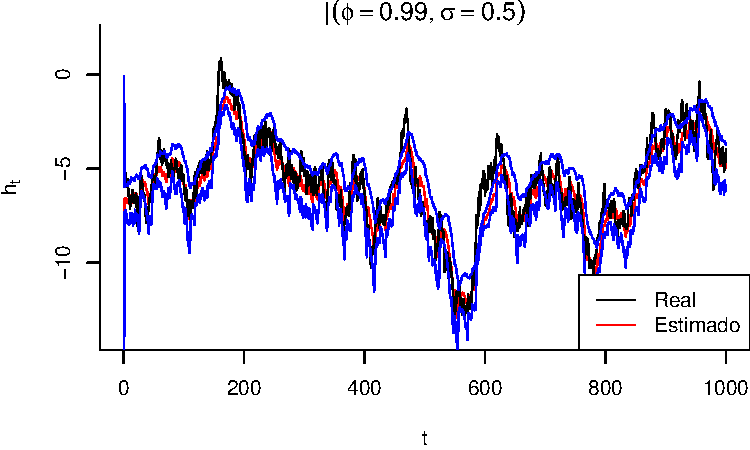
\includegraphics{img/p099s05_inicio}
\end{figure}

Como a própria visualização da série dos valores estimados em relação aos valores reais de $h_t$ sugere, a aplicação da metodologia inspirada em \mccormick\ foi considerada com sucesso, lembrando que os valores reais de $\psi = (\mu, \phi, \sigma^2)$ foram fornecidos ao algoritmo. Então a próxima etapa é juntar esse processo de estimação com o processo iterativo de \kastner.

A primeira execução resultou num erro inesperado já de inicio. O algoritmo para estimar $h_t$ é baseado, por fim, num sorteio de uma distribuição normal com média e variância aproximadas por processos iterativos. Aconteceu que a variância do candidato a $h_t$ foi diminuindo, diminuindo, e após algumas rodadas foi para zero.

O próximo gráfico mostra o que aconteceu com a série estimada da variável latente. O valor inicial é sempre igual a zero, o que funcionou muito bem quando foram fornecidos os valores reais de $\psi = (\mu, \phi, \sigma^2)$, conforme a observação do gráfico anterior. Mas agora, com $\psi$ desconhecido é como se o algoritmo baseado em \mccormick\ caísse num poço de potencial em torno de zero e não conseguisse escapar.

\begin{figure}[ht]
  \centering
  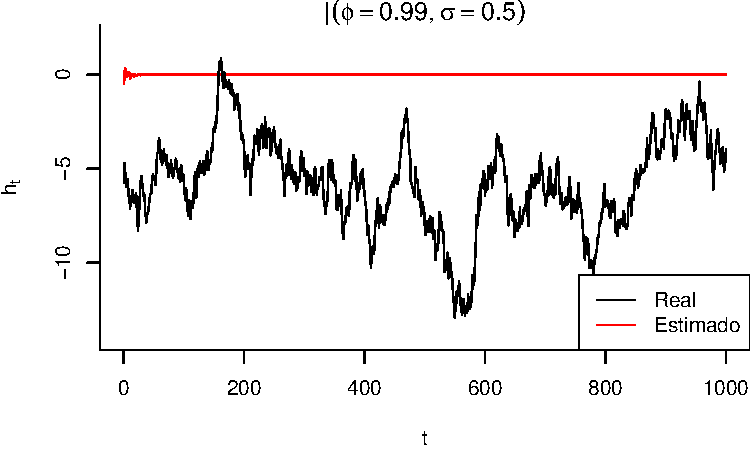
\includegraphics{img/p099s05_1}
\end{figure}

Depois de grande esforço de investigação (testes de tentativa e erro, procura por \textit{bugs} no código e revisão das contas) foi constatado que o parâmetro $\phi$ é extremamente determinante na estimação de $h_t$. O gráfico seguinte mostra o resultado da estimação da variável latente quando todos os parâmetros são desconhecidos, exceto $\phi$. O processo logo após algumas iterações converge para um valor aceitável.

\begin{figure}[ht]
  \centering
  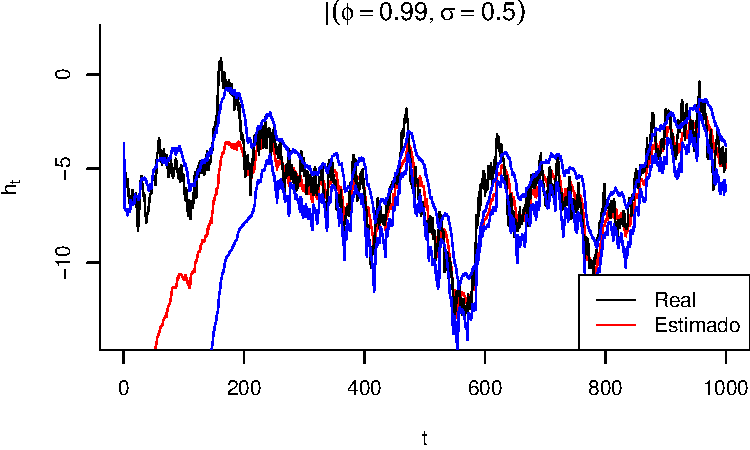
\includegraphics{img/p099s05_2}
\end{figure}

A primeira alternativa, baseada inclusive em outros trabalhos como no próprio \kastner, foi de tomar todos os parâmetros desconhecidos, porém partir do \underline{valor inicial igual ao valor real} do parâmetro (entretanto, nesse caso apenas para $\phi$). Curiosamente o processo voltou a funcionar de forma satisfatória, conforme é mostrado no próximo gráfico, provando mais uma vez a extrema importância de $\phi$ nessa metodologia.

\begin{figure}[ht]
  \centering
  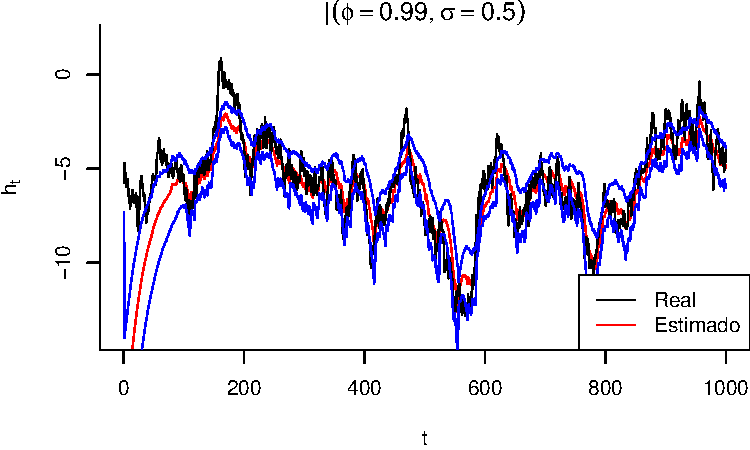
\includegraphics{img/p099s05_3}
\end{figure}

Como iniciar o algoritimo a partir dos valores reais (mesmo que de uma variável apenas) não é uma condição desejável, o plano então foi tentar resolver esse problema da especificação do parâmetro $\phi$.

Após um nova longa jornada de testes computacionais e estudo das equações que definem o problema, surgiu a suspeita de que o termo $R_t = \frac{\phi^2 C_{t-1}}{\lambda_t}$, presente nas derivadas da aproximação tomada no algoritmo, é quem estaria levando para zero a variância do candidato a $h_t$. Então, a proposta natural seria contrabalancear os valores de $\phi$ com $\lambda_t$.

Recapitulando, os valores de $\lambda_t$ foram limitados ao intervalo $(0,8; 1)$. Contudo, em tentativas anteriores, foi percebido que havia uma tendência do fator de desconto, $\lambda_t$, apresentar valores bem pequenos, o que inflacionaria bastante a incerteza das estimativas seguintes. Isso inclusive é a causa de existir esse intervalo limitando os possíveis valores de $\lambda_t$. Então o intervalo limitante foi deixado de lado, e o valor de lambda foi fixado em $0,25$. O resultado pode ser visto nos gráficos seguintes. O primeiro mostra apenas a série real de $h_t$ e os valores médios estimados, enquanto que ao segundo é adicionada a banda de credibilidade de 95\%.

\begin{figure}[ht]
  \centering
  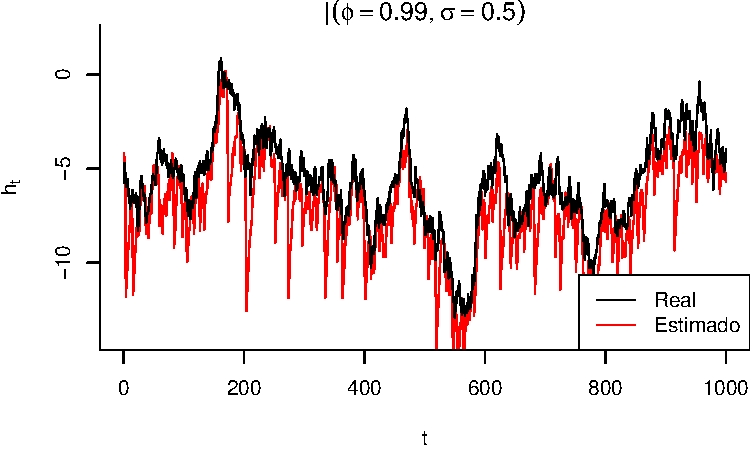
\includegraphics{img/p099s05_4}
\end{figure}

\begin{figure}[ht]
  \centering
  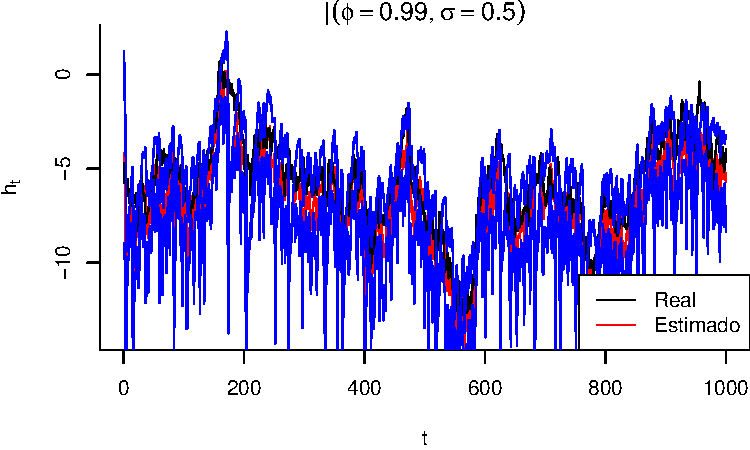
\includegraphics{img/p099s05_5}
\end{figure}

\newpage
É evidente que, como esperado, os valores estimados de $h_t$ ficaram bem mais difusos devido ao baixo valor de $\lambda_t$. Mas agora o algoritmo funcionou sem erros.

Com base nisso os valores estimados dos parâmetros foram calculados para um conjunto de populações com parâmetros pré-fixados, e também pré-fixando $\lambda_t$. O resultados podem ser vistos nos gráficos seguintes. Acima do gráfico estão a média dos valores estimados e entre parêntese o valor real.

O que percebi é que $\mu$ é bem estimado independente das circunstâncias. $\phi$ tem pouquíssima dispersão, mas parece viesado, e aumentar esse viés a medida que o seu valor real decresce, ou fica muito próximo de um. E $\sigma$ tem uma estimativa razoavelmente comportada.

\newpage
\begin{figure}[ht]
  \centering
  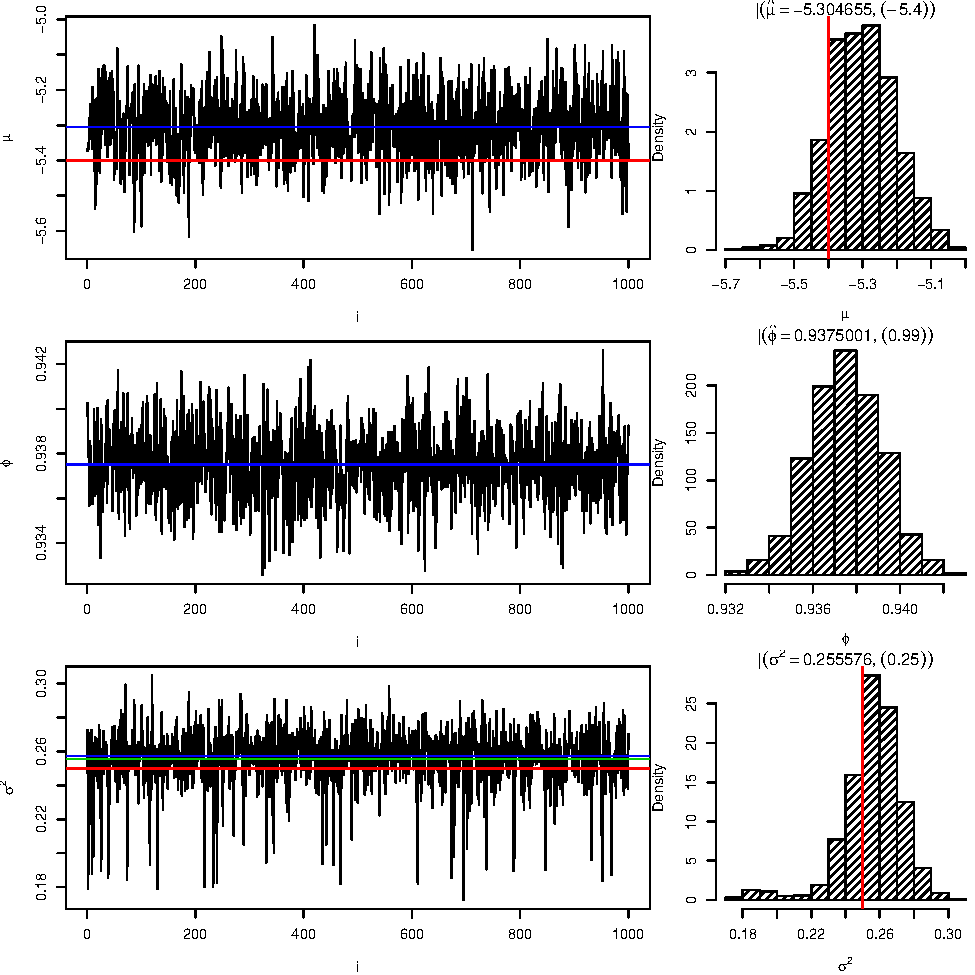
\includegraphics{img/p099s05_result025}
\end{figure}

\newpage
\begin{figure}[ht]
  \centering
  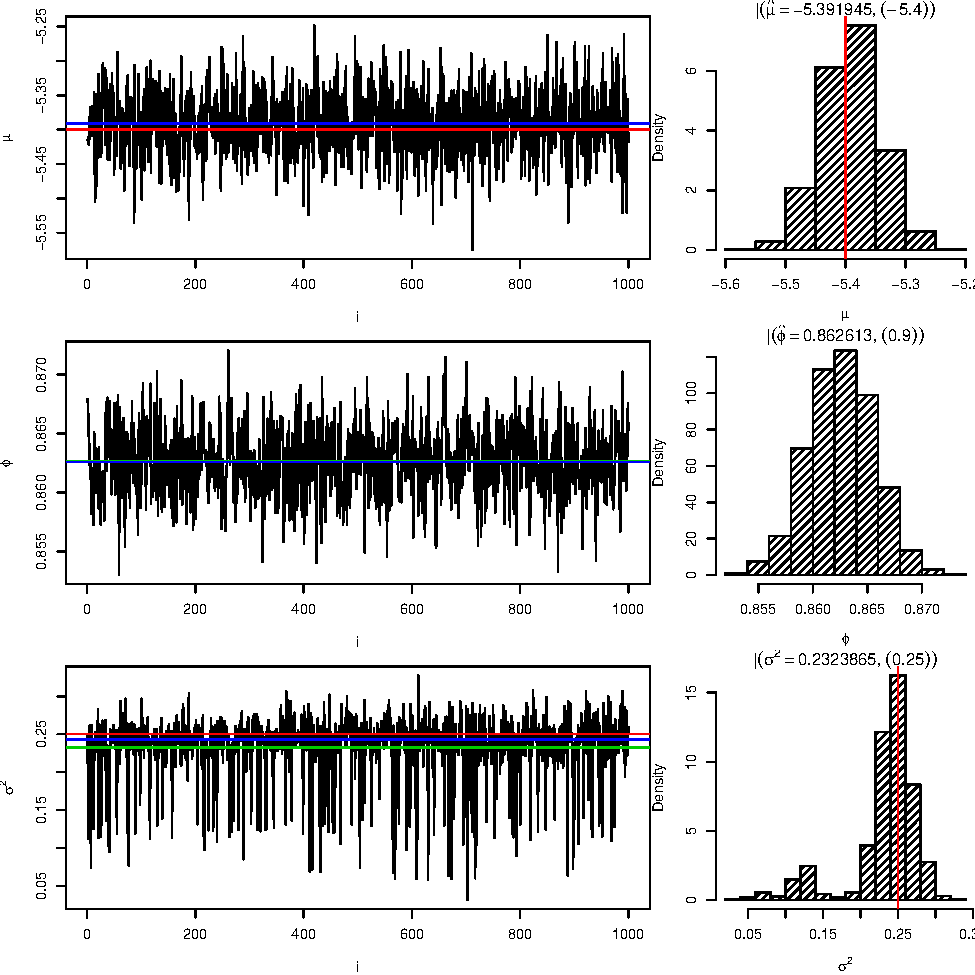
\includegraphics{img/p09s05_result030}
\end{figure}

\newpage
\begin{figure}[ht]
  \centering
  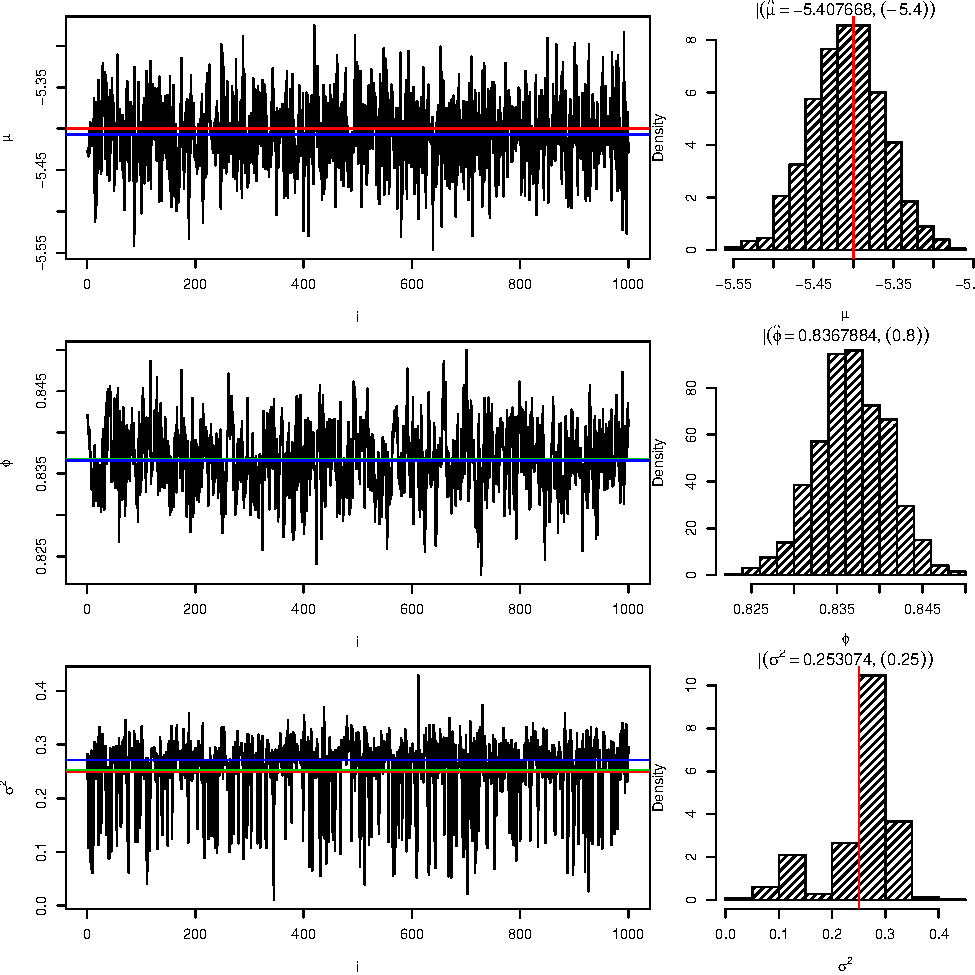
\includegraphics{img/p08s05_result035}
\end{figure}

\newpage
\begin{figure}[ht]
  \centering
  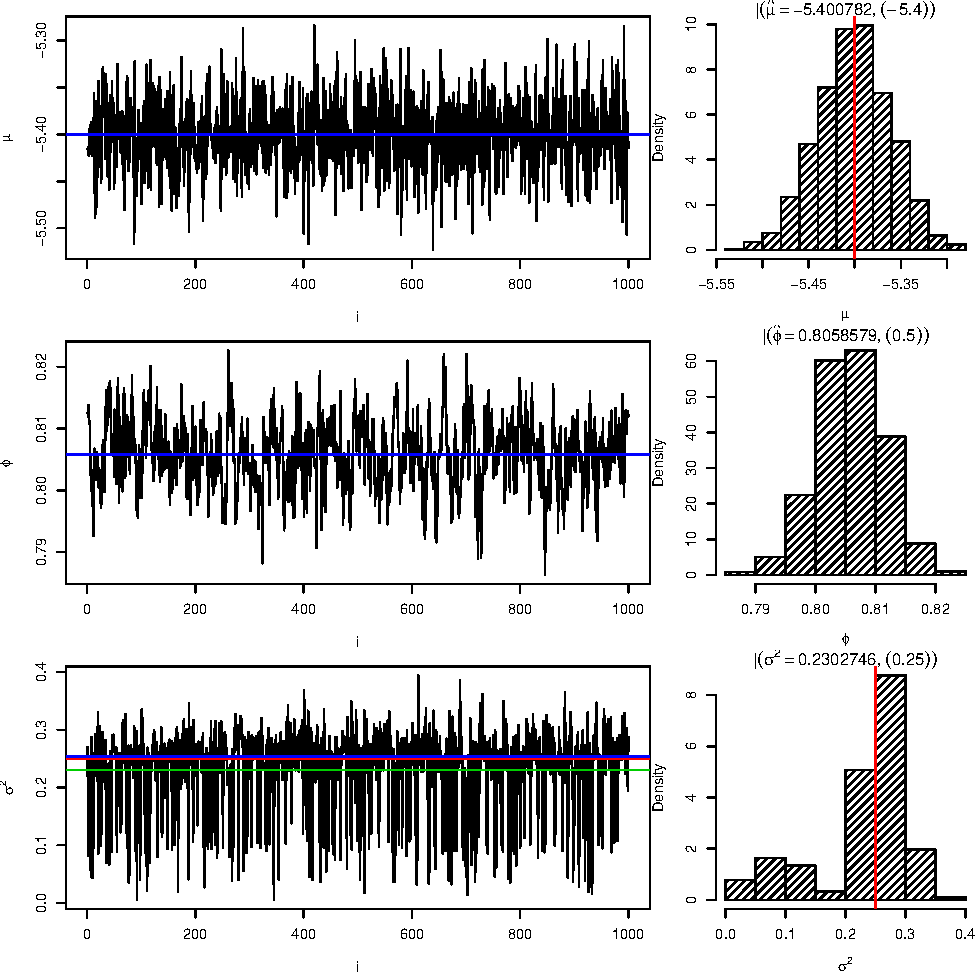
\includegraphics{img/p05s05_result035}
\end{figure}

\newpage
\begin{table}[ht]
  \centering
  \caption{$\mu =-5,4$; $\phi = 0,99$; $\sigma = 0,5$}
  \begin{tabular}{c|rrrrrr|rr}
    \hline
    $\phi_0$ & MAD & MSE & MAPE & SMAPE & MedAPE & MASE & $\bar{\mu}$ & $\bar{\sigma}$\\
    \hline
    0,99 & 2,418 & 9,497 & \textcolor{red}{-1.109,59} & 14,500 & \textcolor{red}{0,397} & 230,40 & -5,331 & 0,203\\
    0,95 & 2,240 & 8,016 & -1.114,87 & 28,490 & 0,400 & 213,45 & -5,306 & 0,244\\
    0,90 & 2,090 & 6,894 & -1.179,27 & -20,236 & 0,559 & 199,15 & -5,301 & 0,293\\
    0,85 & 2,009 & \textcolor{red}{6,312} & -1.228,78 & \textcolor{red}{14,255} & 0,765 & 191,42 & -5,298 & 0,357\\
    0,80 & \textcolor{red}{2,007} & 6,348 & -1.229,54 & 21,681 & 0,844 & \textcolor{red}{191,22} & -5,296 & 0,426\\
    \hline
  \end{tabular}  
\end{table}

\begin{figure}[ht]
  \centering
  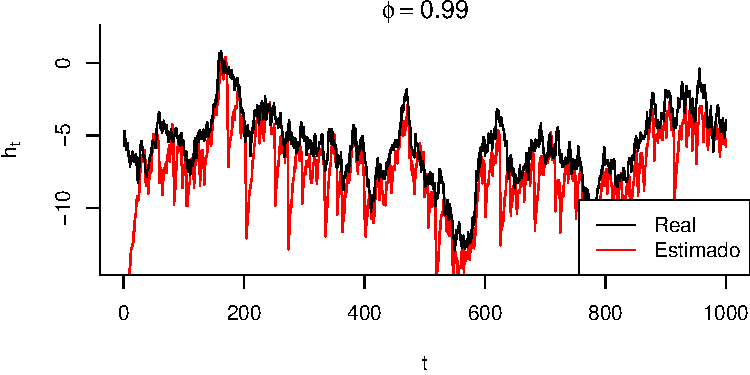
\includegraphics{img/p099s05_final}
\end{figure}

\begin{figure}[H]
  \centering
  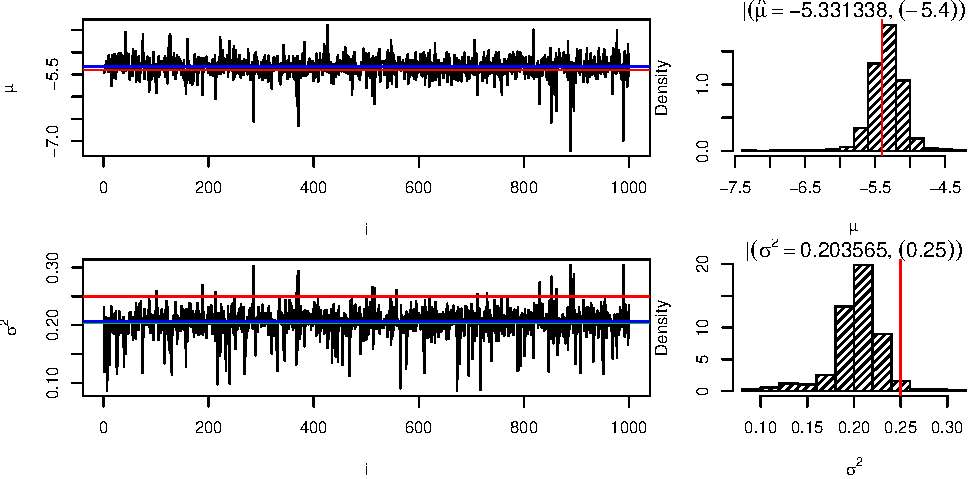
\includegraphics{img/p099s05_resultado}
\end{figure}

\newpage
\begin{table}[ht]
  \centering
  \caption{$\mu =-5,4$; $\phi = 0,9$; $\sigma = 0,5$}
  \begin{tabular}{c|rrrrrr|rr}
    \hline
    $\phi_0$ & MAD & MSE & MAPE & SMAPE & MedAPE & MASE & $\bar{\mu}$ & $\bar{\sigma}$\\
    \hline
    0,99 & 2,450 & 10,395 & -417,81 & 13,961 & -2,332 & 42,02 & -5,404 & 0,043\\
    0,95 & 2,224 & 8,111 & -411,75 & 13,378 & -1,769 & 38,13 & -5,395 & 0,071\\
    0,90 & 2,023 & 6,397 & \textcolor{red}{-353,82} & 12,835 & -1,681 & 34,70 & -5,393 & 0,122\\
    0,85 & 1,892 & 5,572 & -409,72 & 12,464 & \textcolor{red}{-1,225} & 32,44 & -5,391 & 0,173\\
    0,80 & \textcolor{red}{1,802} & \textcolor{red}{5,121} & -419,68 & \textcolor{red}{12,224} & -1,409 & \textcolor{red}{30,90} & -5,391 & 0,225\\
    \hline
  \end{tabular}  
\end{table}

\begin{figure}[ht]
  \centering
  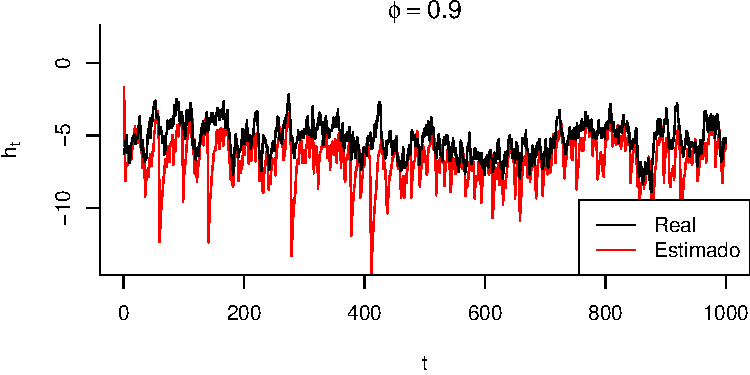
\includegraphics{img/p09s05_final}
\end{figure}

\begin{figure}[H]
  \centering
  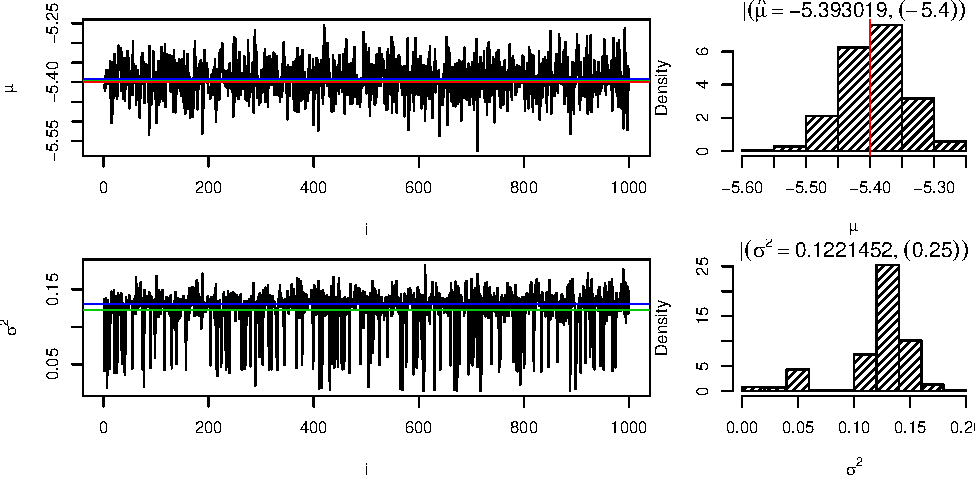
\includegraphics{img/p09s05_resultado}
\end{figure}

\newpage
\begin{table}[ht]
  \centering
  \caption{$\mu =-5,4$; $\phi = 0,8$; $\sigma = 0,5$}
  \begin{tabular}{c|rrrrrr|rr}
    \hline
    $\phi_0$ & MAD & MSE & MAPE & SMAPE & MedAPE & MASE & $\bar{\mu}$ & $\bar{\sigma}$\\
    \hline
    0,99 & 2,287 & 8,519 & \textcolor{red}{-209,19} & 13,287 & -1,670 & -245,88 & -5,422 & 0,053\\
    0,95 & 2,125 & 7,192 & -208,29 & 12,819 & -1,301 & -228,43 & -5,411 & 0,068\\
    0,90 & 1,977 & 6,169 & -212,23 & 12,378 & -1,363 & -212,51 & -5,408 & 0,085\\
    0,85 & 1,855 & 5,422 & -216,79 & 12,022 & -1,135 & -199,42 & -5,407 & 0,106\\
    0,80 & \textcolor{red}{1,758} & \textcolor{red}{4,892} & -214,75 & \textcolor{red}{11,754} & \textcolor{red}{-0,92} & \textcolor{red}{-189,01} & -5,406 & 0,147\\
    \hline
  \end{tabular}  
\end{table}

\begin{figure}[ht]
  \centering
  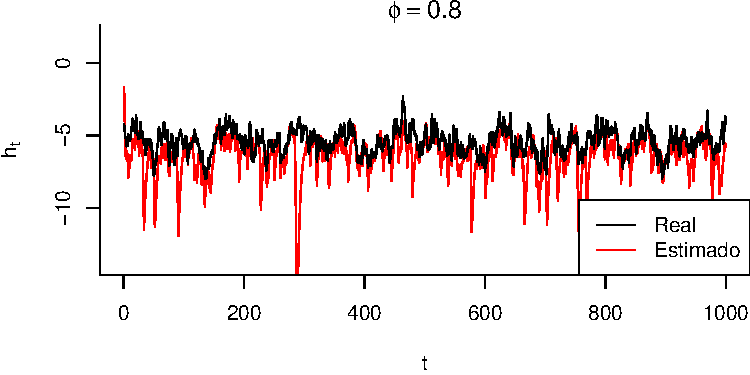
\includegraphics{img/p08s05_final}
\end{figure}

\begin{figure}[H]
  \centering
  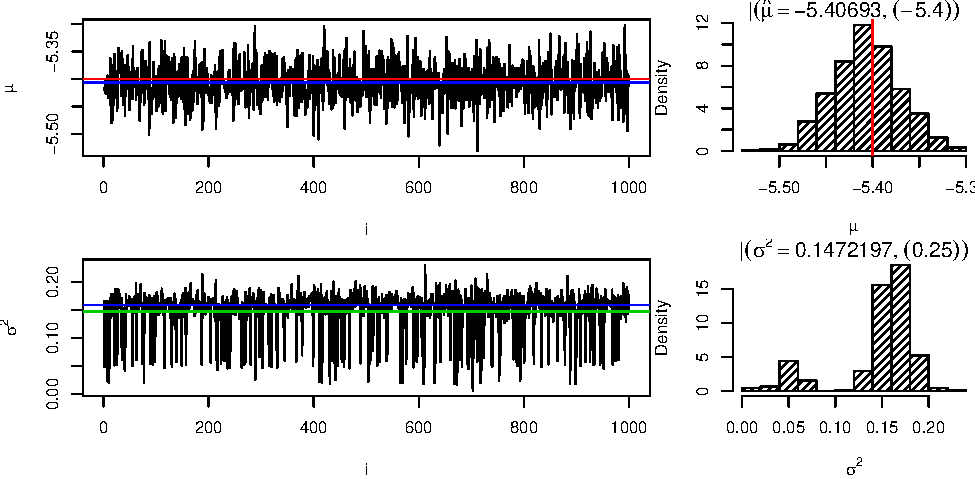
\includegraphics{img/p08s05_resultado}
\end{figure}

\end{document}
